\documentclass[a4paper, 12pt]{scrartcl}

\usepackage[english]{babel}
\usepackage[utf8]{inputenc}
\usepackage{amsmath}
\usepackage{geometry}
\usepackage{caption}
\usepackage{graphicx}
\usepackage[colorinlistoftodos]{todonotes}
\usepackage{hyperref}
\usepackage{booktabs}
\usepackage{cleveref}
\usepackage{listings}
\usepackage{listings-golang}
\usepackage{makecell}
\usepackage{sectsty}
\usepackage{comment}
\usepackage{multicol}

\let\bold\textbf
\setlength\parindent{0pt}
% \todo[inline]{Add diagram here}

\title{\vspace{40mm}CS628 Assignment 1 \\ $2018\text{-}19$  II Semester \\ \vspace{1cm} \textbf{Design Report for Secure Key-Value File Sharing}}
\subtitle{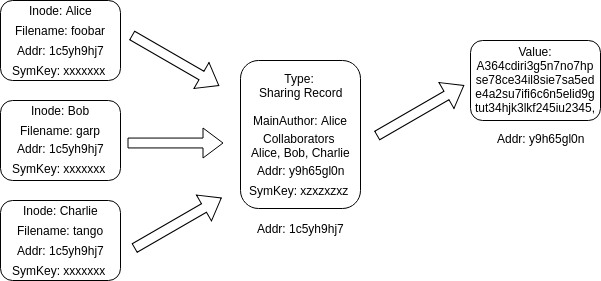
\includegraphics[width=\textwidth, height=7cm]{cs628.png}\vspace{20mm}}
\author{Aniket Pandey $(160113)$ $\cdot$ Ashish Kumar $(160160)$}
\date{\today}

\geometry{
a4paper,
total={180mm,260mm},
left=15mm,
top=15mm,}

%\sectionfont{\fontsize{15}{15}\selectfont}
%
%\title{%
%   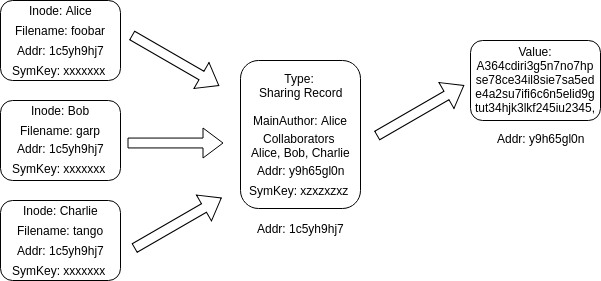
\includegraphics[width=13cm, height=5cm]{cs628.png}
%}

\begin{document}
\clearpage\maketitle
\thispagestyle{empty}
\newpage

%\begin{center}
%	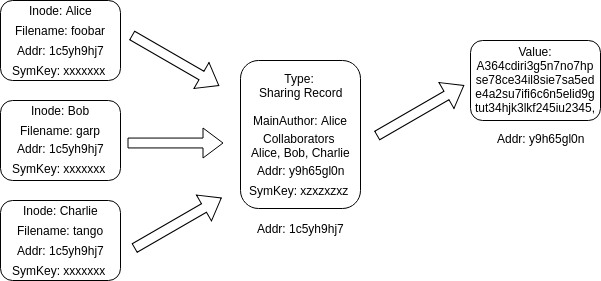
\includegraphics[width=13cm, height=5cm]{cs628.png}
%\end{center}

\section{A simple, but secure client}
Main Purpose: To maintain Confidentiality and Integrity of data without any regards to Availability.

\begin{multicols}{2}

\begin{center}
	\textbf{USER Structure}
\end{center}

\begin{center}
	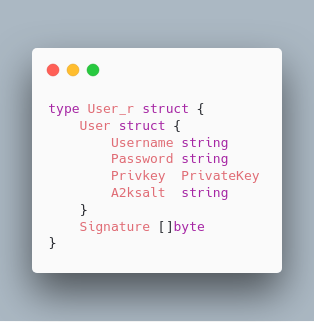
\includegraphics[width=7cm, height=5cm]{user.png}
\end{center}

\columnbreak

\begin{center}
	\textbf{INODE Structure}
\end{center}

\begin{center}
	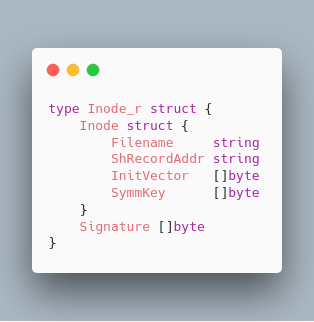
\includegraphics[width=7cm, height=5cm]{inode.png}
\end{center}

\end{multicols}

\subsection{InitUser (username string, password string)}
\begin{enumerate}
	\itemsep0em

	\item Obtain $key = Argon2Key("<username>+user", "<password>+pass", 10)$. This will generate a 36 character key. This is where the value (User data) will be stored.
	\item Generate an RSA Key-pair. Push the public key to the Public Key Server. Private key stored.
	\item Obtained the HMAC signature of User struct. Encrypt the json-marshalled User\_r struct data with AES-Cipher Feedback Mode. The "key" for CFBEncrypter() is obtained via Argon2key(), with salt="$<$password$>$+ssap" while password is same as above.
	\item Call $DatastoreSet(key, ciphertext)$ to publish the encrypted User information in Data Server.
\end{enumerate}

\subsection{GetUser (username string, password string)}
\begin{enumerate}
	\itemsep0em

	\item Get the "key" using above Argon2Key invocation. Errors suggest either incorrect username or password. Calculate the key for CFBDecrypter(), and obtain the decrypted User\_r structure.
	\item Check HMAC hashes of $User\_r.User$ and $User\_r.Signature$ for any tampering. \textbf{Confirm} if the passwords match. 
	\item If all checks are satisfied, return the $User\_r.User$ structure.
\end{enumerate}

\subsection{(User) StoreFile (filename string, data []byte)}
\begin{enumerate}
	\itemsep0em
	\item Obtain $key = Argon2Key("<username>+<filename>", "<password>+<filename>", 10)$. This will generate a 36 character key. This is where the Inode structure for "Username"-"Filename" will be stored (Refer to the figure).
	\item Generate a random address (key) and AES-CFB key for storing and encrypting SharingRecord\_r structure respectively. Fill the Inode structure. Sign it using Author's Private key and store RSA signature in $Inode\_r.Signature$. Encrypt $Inode\_r$ with Author's Public key. Push (key, encrypted Inode\_r) to Data Server.
	\item Initialize a SharingRecord\_r structure. Fill up all values. Add original author to Collaborators. \textbf{NOTE:} The List of Collaborators is most important construct in this design. Explained ahead.
	\item Again generate a random address (key) and AES-CFB key for storing and encrypting the $Data\_r$ structure. Store these in the relevant fields of SharingRecord structure. Sign with a predecided HMAC key and store in $SharingRecord_r.Signature$ field. Encrypt the Structure with the key decided at $Inode_r$ and push to Data Server.
	\item Store the "data" at The key generated above, Encrypt it with CFBEncrypter() method. Sign it and store the data at the "key". Push to Data Server and return. 
\end{enumerate}

\subsection{(User) LoadFile (filename string)}
\begin{enumerate}
	\itemsep0em
	\item Follow the method given in StoreFile() to reach, decrypt and verify the signature of the Inode structure corresponding to "filename". 
	\item \textbf{IMP:} Check if $User_r.User.username$ is in Collaborators. If so, continue following the method in StoreFile to get to the Data location, decrypt the data, verify the signature and return it.
\end{enumerate}

\subsection{(User) AppendFile (filename string, data []byte)}
\begin{enumerate}
	\itemsep0em
	\item Follow the method given in LoadFile() to reach, decrypt and verify the signature of the $Data\_r$ structure corresponding to "filename". 
	\item \textbf{NOTE:} Using the property of Cipher Feedback Mode, we don't need to decrypt the entire data for append operation. Instead, using the stored CipherText as Initialization vector, we can continue the encryption operation more efficiently.
	\item Recalculate the signature and push the modifed data to Data Server.
\end{enumerate}

\section{Sharing and revocation}

\subsection{(User) ShareFile (filename string, recipient string)}
\begin{enumerate}
	\itemsep0em
	\item Follow the method given in LoadFile() to reach, decrypt and verify the signature of the $SharingRecord\_r$ structure corresponding to "filename". \textbf{IMP} Verify if the user is present in Collaborators.
	\item Collect the address and AES-CFB encryption key of $SharingRecord\_r$ structure from the respective Inode. Recieve the Public key of receiver from the Public Key Server.
	\item $sharing = PrivKey_{User}(PubKey_{recipient}(Collected Info))$, to maintain confidentiality and integrity in case of a \textbf{Man in the Middle attack} while sharing the message offline.
\end{enumerate}

\subsection{(User) ReceiveFile (filename string, sender string, msgid string)}
\begin{enumerate}
	\itemsep0em
	\item Decrypt "msgid" using Private Key of User, verify the integrity using Public Key of Sender. Obtain the Address and "key" for CFB-Decryption of SharingRecord structure of the concerned data(value).
	\item \textbf{IMP} Check if the sender is in Collaborators. If so, proceed ahead.
	\item Create an Inode for the receiver user using Argon2Key, with the method described in StoreFile(). Store the info in the Inode, store the RSA signature and encrypt $Inode\_r$ structure with Public key of User. Return.
\end{enumerate}

\subsection{(User) RevokeFile (filename string)}
\begin{enumerate}
	\itemsep0em
	\item Go to the SharingRecord structure corresponding to "filename". \textbf{IMP} After verifying the integrity, check if the User is \textbf{Original-Author} of the "filename".
	\item If so, clear the list of collaborators except the original-author. From the Inode of original author, change the encryption key of SharingRecord structure and re-encrypt it with a new key. \textbf{NOTE:} This is to prevent any further invocation of "RevokeFile()" method by a distrusted user.
\end{enumerate}


\end{document}
